\chapter{Data}
\label{cha:data}

\section{Data acquisition}
\label{sec:data-acquisition}

The data was acquired at the \acrfull{sas} laboratory at Linköping University. The experiment --- as shown in Figure~\ref{fig:experimental-setup} --- consisted of exposing different gas combinations to two \acrshort{sicfet} sensors under a particular frequency cycle and recording its response, measured in \acrfull{ma}. The response is then used to extract secondary features, namely average and slope values from certain regions of the frequency cycle. These shape-defining features were not chosen randomly; they are staples in the literature and are promising to this type of problem \parencite{Bastuck_2019} \parencite{Bur791934}.

\begin{figure}[!htb]
	\centering
	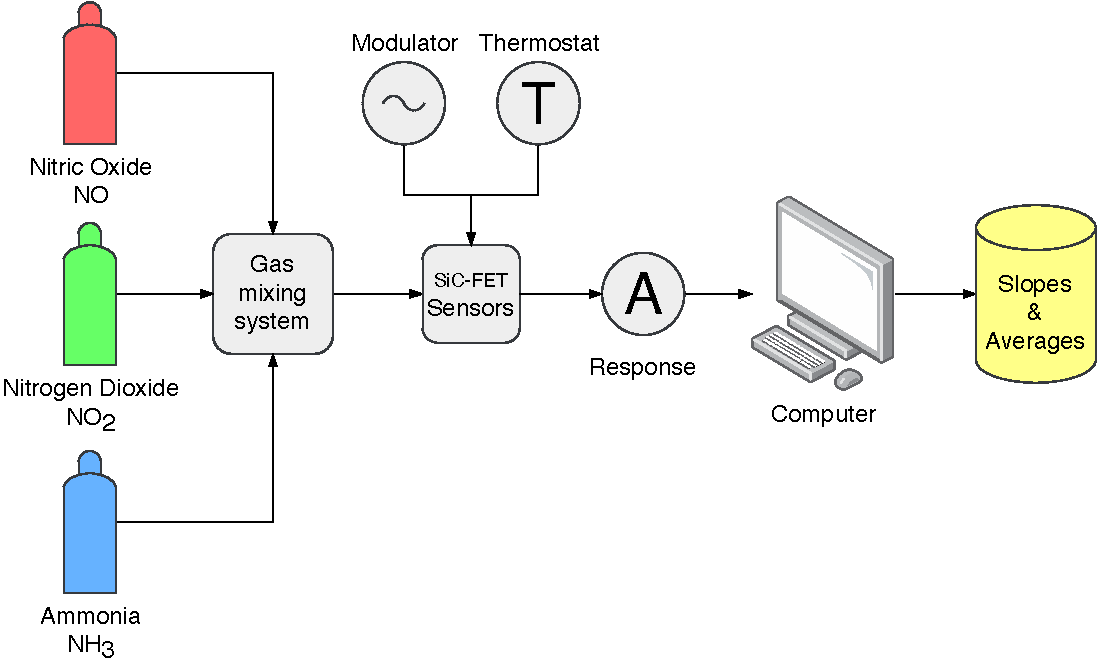
\includegraphics[width=0.8\textwidth]{../figures/experimental-setup.pdf}
	\caption{Schema of the data acquisition process.}
	\label{fig:experimental-setup}
\end{figure}

In more detail, \ch{NO}, \ch{NO2} and \ch{NH3} had five possible concentration values each: 5, 10, 20, 40, and 80 \acrfull{ppm}. The experiment was designed to encompass all possible combinations of these gases, amounting to 125 different gas mixtures. Each feature was submitted to the same frequency cycle four times. The cycle consists of 16 unique frequencies: 0.05, 0.1, 0.25, 0.5, 1, 2, 5, 10, 25, 50, 100, 200, 500, 1000, 2500 and 5000 \acrfull{hertz}. A typical raw sensor response for frequency modulation experiments is shown in Figure~\ref{fig:raw}.

\begin{figure}[!htb]
	\centering
	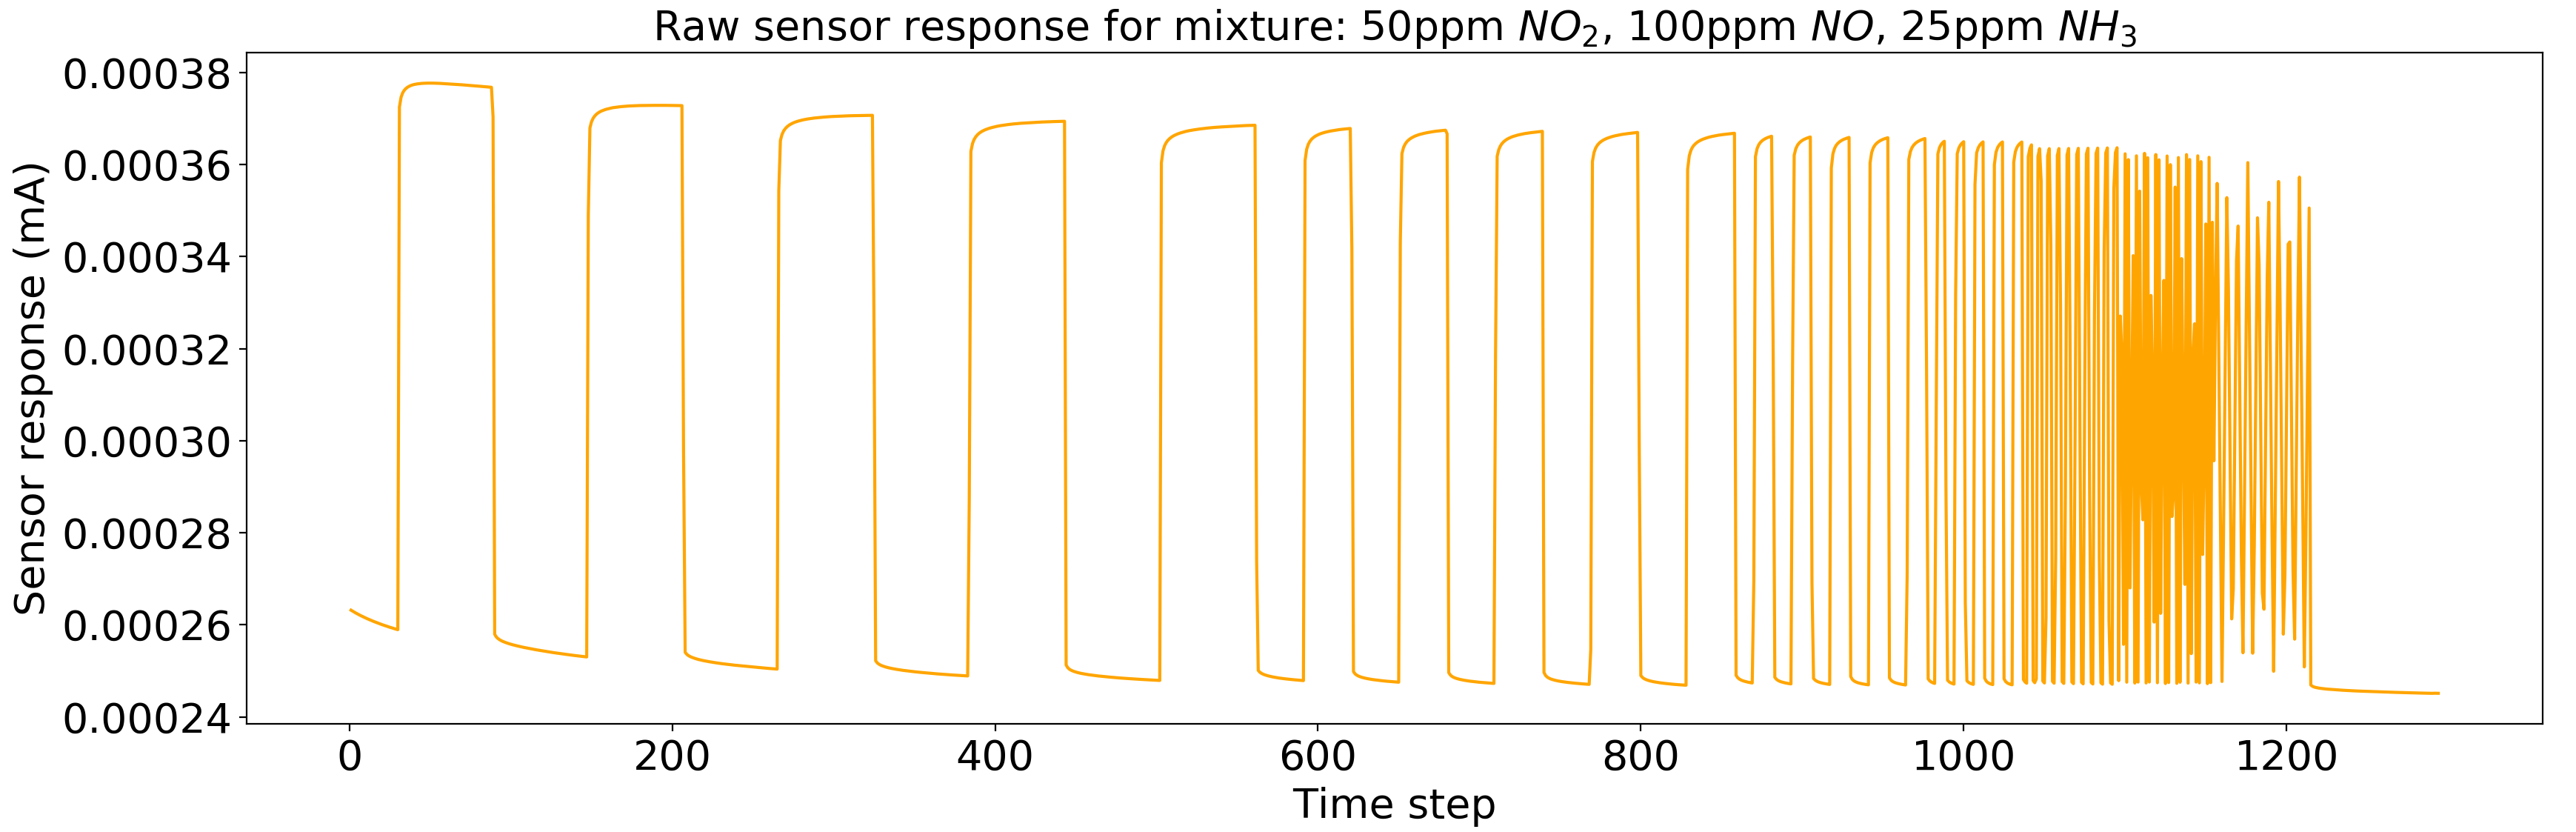
\includegraphics[width=1\textwidth]{../figures/raw-response.png}
	\caption{An example of raw sensor response}
	\label{fig:raw}
\end{figure}

Throughout one cycle, several slope and average features were extracted. The sample rate for feature extraction was set at 4 \acrshort{hertz}, i.e. in a cycle of 60 seconds, a total of $60 \text{s} \times 4 \frac{1}{\text{s}} = 240$ pairs of slopes and averages are recorded, which totals to 480 features per cycle. In other words, during one experiment --  4 cycles of 60 seconds -- a total of $480 \times 4 = 1920$ features are extracted. 

One way to visualize the above process is shown in Figures~\ref{fig:feat-window}. Note that the y-axis is in log-scale due to the different orders of magnitude of frequencies. Moreover, Figure~\ref{fig:features} gives more insight into feature measurement, and Table~\ref{tab:measurements} summarizes the data acquisition details.

\hspace{2mm}

\begin{figure}[!htb]
	\centering
	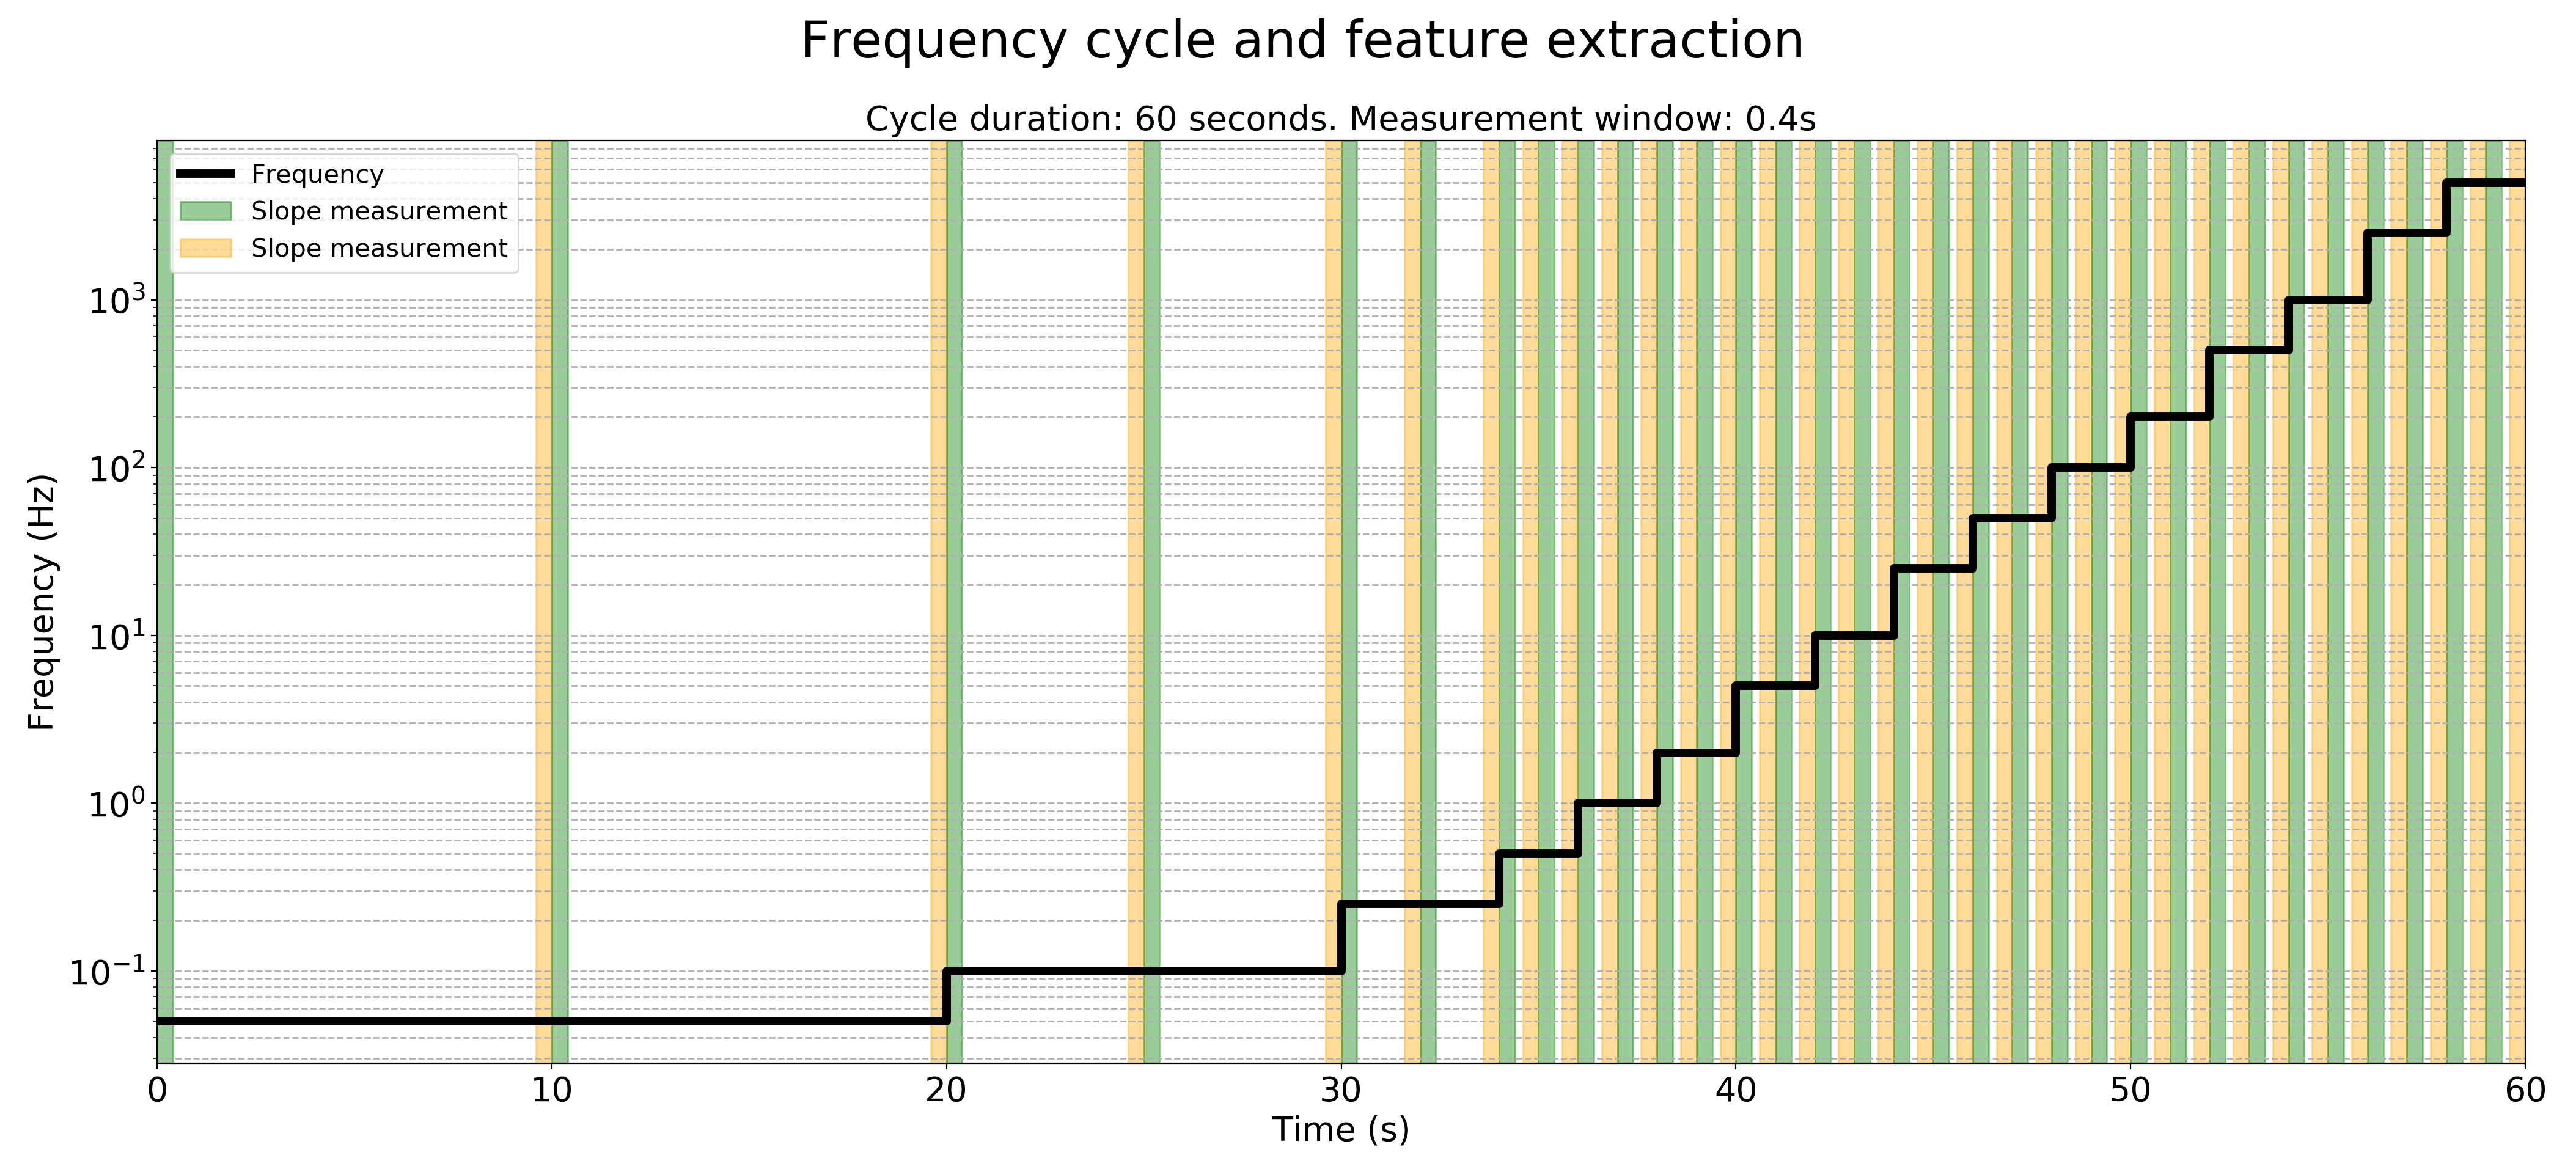
\includegraphics[width=0.9\textwidth]{../figures/measurement-windows.png}
	
	\caption{Feature measurements times per cycle. The width of the red line indicates the duration of one of the feature measurement windows as an example.}
	\label{fig:feat-window}
\end{figure} 

\begin{figure}[h]
	\centering
	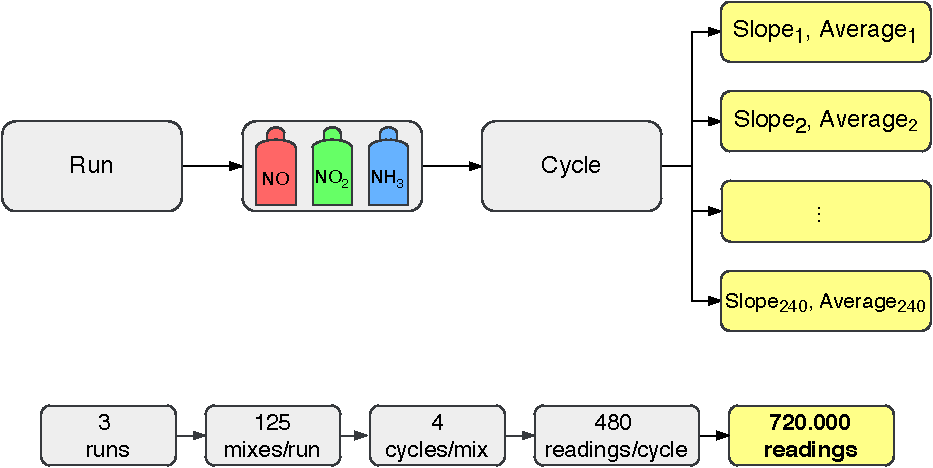
\includegraphics[width=0.9\textwidth]{../figures/features.pdf}
	\caption{A visualization of the feature measurement process.}
	\label{fig:features}
\end{figure}


\begin{table}[!ht]
	\centering
	\caption{Data acquisition details}
	\label{tab:measurements}
	\begin{tabular}{|c|c|}
		\hline
		\textbf{Parameter} & \textbf{Value} \\
		\hline
		Factors (gases) & 3 \\
		\hline
		Levels (concentrations) & 5 \\
		\hline
		Frequencies & 16 \\
		\hline
		Features per cycle & 480 \\
		\hline
		Number of cycles & 4 \\
		\hline
		Data points per mixture & 1920\\
		\hline
		Number of mixtures & 125 \\
		\hline
		Features per experiment & 240.000 \\
		\hline
		Number of experiments & 3 \\
		\hline
		Total features & 720.000 \\
		\hline
	\end{tabular}
\end{table}

For specific timestamps and measurements duration, the reader is referred to Appendix~\ref{app:A}.

\newpage
\section{Raw data}
\label{sec:raw-data}

The experiments were run between 26th and 29th March 2021. The experiment data was exported as an excel file containing twelve columns, as specified in Tables~\ref{tab:raw-cols} and \ref{tab:raw-sample}.

\begin{table}[h]
	\centering
	\caption{Raw data column details}
	\label{tab:raw-cols}
	
	\resizebox{\textwidth}{!}{%
		\begin{tabular}{|c|c|c|}
		\hline
		\textbf{Name} & \textbf{Description} & \textbf{Unit} \\
		\hline
		Exposure nr & A particular mix of NO, NO$_2$ and NH$_3$. Ranges from 1 to 375  & -\\
		\hline
		Cycle nr & The cycle number. Ranges from 1 to 4. & - \\
		\hline
		Sample nr & Extracted feature index. Ranges from 1 to 240 & - \\
		\hline
		NO & Nitric Oxide concentration & \acrshort{ppm} \\
		\hline
		NO2 & Nitrogen Dioxide concentration &\acrshort{ppm} \\
		\hline
		NH3 & Ammonia concentration &\acrshort{ppm} \\
		\hline
		Freq & Frequency & \acrshort{hertz}\\
		\hline
		Slope sensor 1 & Slope & $\mu$A/s \\
		\hline
		Slope sensor 2 & Slope & $\mu$A/s\\
		\hline
		Average sensor 1 & Average & $\mu$A \\
		\hline
		Average sensor 2& Average & $\mu$A\\
		\hline
		Sensor temperature & Temperature & degrees Celsius ($^{\circ}$C) \\
		\hline
	\end{tabular}}
\end{table}

\begin{table}[h]
	\centering
	\caption{Sample of raw data.}
	\label{tab:raw-sample}
	\resizebox{\textwidth}{!}{%
		\begin{tabular}{p{1.5cm}p{1.3cm}p{0.8cm}p{1.3cm}p{0.8cm}p{0.8cm}p{1.8cm}p{1.8cm}p{1.8cm}p{1.8cm}p{1.8cm}p{1.8cm}p{1.8cm}}
		\toprule[0.5mm]
		Index & Exposure\newline nr &  Cycle\newline  nr &  Sample\newline  nr &  NO\newline  [ppm] &  NO2\newline  [ppm] &  NH3\newline  [ppm] &  Freq\newline  [Hz] &  Slope\newline  sensor 1\newline [$\mu$A/s] &  Slope\newline  sensor 2\newline [$\mu$A/s] &  Average\newline  sensor 1\newline [$\mu$A] &  Average\newline  sensor 2\newline [$\mu$A] &  Sensor\newline  temperature \newline[C] \\
		\midrule[0.5mm]
		0 &            1 &         1 &          1 &        10 &          5 &         20 &       0.05 &             -18.855169 &             -22.588416 &                32.926184 &                27.961554 &              274.994683 \\
		1 &            1 &         1 &          2 &        10 &          5 &         20 &       0.05 &             -28.289268 &             -28.185027 &                25.853867 &                20.915297 &              274.980487 \\
		2 &            1 &         1 &          3 &        10 &          5 &         20 &       0.05 &              -0.390916 &              -0.482129 &                25.756138 &                20.794765 &              274.985895 \\
		3 &            1 &         1 &          4 &        10 &          5 &         20 &       0.05 &              -0.234549 &              -0.156366 &                25.697501 &                20.755673 &              275.020372 \\
		4 &            1 &         1 &          5 &        10 &          5 &         20 &       0.05 &              -0.143336 &              -0.247580 &                25.661667 &                20.693778 &              275.014964 \\
		
		\bottomrule
		&&&&&&&&&&&&\\
		&&&&&&&\sbox0{\dots}\makebox[\wd0]{\vdots}&&&&&\\
		&&&&&&&&&&&&\\
		\toprule
		
		100000 &          105 &         1 &        161 &         5 &          5 &         40 &        5.0 &             -38.366212 &             -48.495271 &                30.241896 &                24.821197 &              275.021724 \\
		100001 &          105 &         1 &        162 &         5 &          5 &         40 &        5.0 &               6.619507 &               8.521964 &                31.896773 &                26.951688 &              274.999415 \\
		100002 &          105 &         1 &        163 &         5 &          5 &         40 &        5.0 &              -1.941549 &               6.580416 &                31.411386 &                28.596792 &              275.011584 \\
		100003 &          105 &         1 &        164 &         5 &          5 &         40 &        5.0 &              27.401023 &              22.012900 &                38.261641 &                34.100017 &              275.009894 \\
		100004 &          105 &         1 &        165 &         5 &          5 &         40 &        5.0 &             -27.016623 &             -28.439121 &                31.507486 &                26.990236 &              275.014400 \\
		\bottomrule
		&&&&&&&&&&&&\\
		&&&&&&&\sbox0{\dots}\makebox[\wd0]{\vdots}&&&&&\\
		&&&&&&&&&&&&\\
		\toprule
		
		359995 &          375 &         4 &        236 &        20 &         80 &          5 &     5000.0 &              -0.136821 &              -0.158538 &                34.129879 &                30.345597 &              275.002007 \\
		359996 &          375 &         4 &        237 &        20 &         80 &          5 &     5000.0 &               0.010859 &               0.010859 &                34.132593 &                30.348312 &              274.986797 \\
		359997 &          375 &         4 &        238 &        20 &         80 &          5 &     5000.0 &              -0.043435 &               0.030405 &                34.121734 &                30.355913 &              274.979811 \\
		359998 &          375 &         4 &        239 &        20 &         80 &          5 &     5000.0 &              -0.117275 &              -0.026061 &                34.092416 &                30.349398 &              274.984543 \\
		359999 &          375 &         4 &        240 &        20 &         80 &          5 &     5000.0 &               0.073840 &               0.039092 &                34.110876 &                30.359171 &              274.998063 \\
		\bottomrule[0.5mm]
	\end{tabular}}
\end{table}

\newpage
\section{Pre-processing}
\label{sec:preprocessing}

The features (slopes and averages) from the same target (a particular exposure) in the raw data file in Table~\ref{tab:raw-sample} are spread across multiple rows, which is not suitable for analysis, as different features from the same observation as spread along multiple columns. As opposed to \acrshort{tco}, the experiments were conducted at constant temperature, and therefore, the temperature column is discarded. The data was, subsequently, modified to have the desired format: each row containing the predictors for one particular combination of gases. Additionally, the data from each sensor was split into  two datasets. 

The naming convention for the features is shown in Figure~\ref{fig:feat-naming}. First, the frequency in which the measurement was taken followed by the sensor number. After that, the feature name itself is followed by its index, i.e. where in the frequency cycle the measurement was made. This convention allows for easy identification of key information of the cycle and measurement.

\begin{figure}[h]
	\centering
	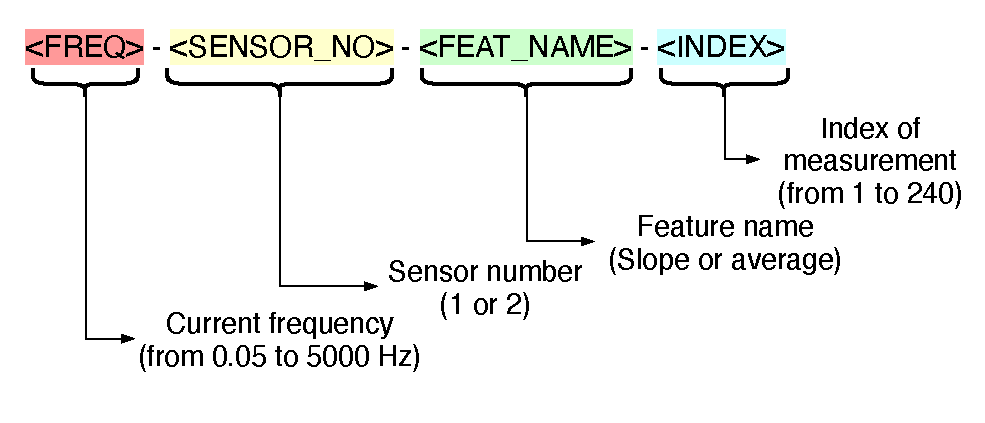
\includegraphics[width=1\textwidth]{../figures/feat-naming.pdf}
	\caption{Feature naming convention.}
	\label{fig:feat-naming}
\end{figure}

The pre-processing results in the format shown in Figure~\ref{fig:preprocessed-data}. Recalling that there are 125 possible mixtures of gases, it is important to note that there are repeated exposures in the data set, and those are treated as individual observations. Since each unique gas mixture was exposed 4 times during a cycle, and the experiment was repeated 3 times, this yields a total of $4 \times 3 \times 125 = 1500$ exposures. A snippet of the final data set is shown in Table~\ref{tab:prepro-sample}.

\begin{figure}[h]
	\centering
	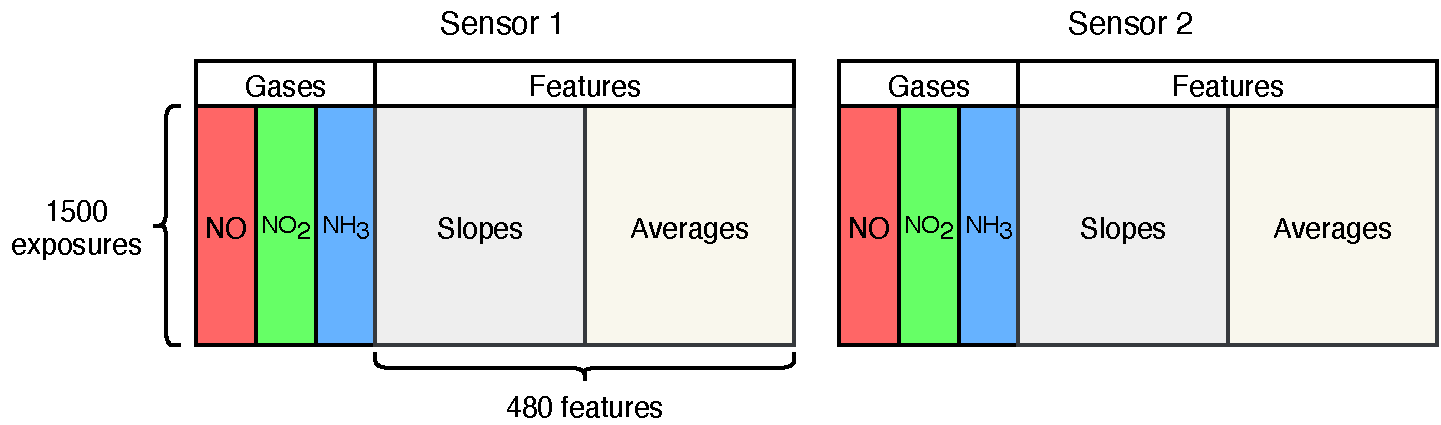
\includegraphics[width=1\textwidth]{../figures/preprocessed-data.pdf}
	\caption{Pre-processed data structure.}
	\label{fig:preprocessed-data}
\end{figure}

\begin{table}
	\centering
	\caption{Sample of pre-processed data.}
	\label{tab:prepro-sample}
	\resizebox{\textwidth}{!}{%
	\begin{tabular}{ccp{0.8cm}p{0.8cm}p{0.8cm}p{1.8cm}p{1.8cm}p{0.3cm}p{1.6cm}p{1.6cm}p{1.6cm}p{1.6cm}p{0.3cm}p{1.6cm}p{1.6cm}}
		\toprule[0.5mm]
		Index &  EXPOSURE &    NO &   NO2 &   NH3 &  0.05-1-slope-0 &  0.05-1-slope-1 & $\dots$&  5000.0-1-slope-239 &  0.05-1-avg-0 &  0.05-1-avg-1 &  0.05-1-avg-2 & $\dots$&  5000.0-1-avg-238 &  5000.0-1-avg-239 \\
		\midrule[0.5mm]
		0 &       1.0 &  10.0 &   5.0 &  20.0 &      -18.855169 &      -28.289268 &$\dots$&            0.019546 &     32.926184 &     25.853867 &     25.756138 &$\dots$&         35.840135 &         35.845021 \\
		1 &       1.0 &  10.0 &   5.0 &  20.0 &      -28.979886 &       -9.251672 &$\dots$&           -0.056466 &     28.600050 &     26.287132 &     26.225237 & $\dots$&        35.884113 &         35.869996 \\
		2 &       1.0 &  10.0 &   5.0 &  20.0 &      -25.431240 &      -12.874158 &$\dots$&           -0.052122 &     29.512187 &     26.293647 &     26.238267 & $\dots$&        35.913432 &         35.900401 \\
		3 &       1.0 &  10.0 &   5.0 &  20.0 &      -30.126572 &       -8.196200 &$\dots$&           -0.156366 &     28.368758 &     26.319708 &     26.254555 &$\dots$&         35.939493 &         35.900401 \\
		4 &       2.0 &  20.0 &  40.0 &  40.0 &      -19.506695 &      -27.051368 & $\dots$&          -0.078183 &     33.180279 &     26.417437 &     26.303420 &$\dots$&         35.685397 &         35.665852 \\
		\bottomrule
		&&&&&&&&&&&&&&\\
		&&&&&&&\sbox0{\dots}\makebox[\wd0]{\vdots}&&&&&&&\\
		&&&&&&&&&&&&&&\\
		\toprule
		
		700 &     176.0 &  40.0 &  20.0 &  40.0 &      -21.011721 &      -25.822155 &$\dots$&            -0.071668 &     31.458621 &     25.003082 &     24.902639 & $\dots$&         34.554999 &         34.537082 \\
		701 &     176.0 &  40.0 &  20.0 &  40.0 &      -27.505265 &      -10.847911 &$\dots$&             0.086870 &     27.660766 &     24.948788 &     24.918927 & $\dots$&         34.504506 &         34.526224 \\
		702 &     176.0 &  40.0 &  20.0 &  40.0 &      -27.516124 &      -10.750182 &$\dots$&            -0.097729 &     27.647193 &     24.959647 &     24.928700 & $\dots$&         34.531653 &         34.507221 \\
		703 &     176.0 &  40.0 &  20.0 &  40.0 &      -27.364102 &      -10.875058 &$\dots$&             0.086870 &     27.666195 &     24.947431 &     24.935215 & $\dots$&         34.537082 &         34.558800 \\
		704 &     177.0 &  80.0 &  40.0 &  40.0 &      -20.794546 &      -26.195696 &$\dots$&             0.041263 &     31.640505 &     25.091581 &     25.088324 &$\dots$&          34.695078 &         34.705393 \\
		
		\bottomrule
		&&&&&&&&&&&&&&\\
		&&&&&&&\sbox0{\dots}\makebox[\wd0]{\vdots}&&&&&&&\\
		&&&&&&&&&&&&&&\\
		\toprule
		
		1495 &     374.0 &  80.0 &  80.0 &  40.0 &      -27.937445 &      -10.891346 &$\dots$&            -0.097729 &     27.166692 &     24.443855 &     24.392276 &$\dots$&          34.151596 &         34.127164 \\
		1496 &     375.0 &  20.0 &  80.0 &   5.0 &      -24.358394 &      -22.933723 &$\dots$&            -0.008687 &     30.315735 &     24.582305 &     24.530726 &$\dots$&          34.134765 &         34.132593 \\
		1497 &     375.0 &  20.0 &  80.0 &   5.0 &      -28.862612 &       -9.827186 &$\dots$&            -0.112931 &     26.916940 &     24.460144 &     24.410736 &$\dots$&          34.159740 &         34.131507 \\
		1498 &     375.0 &  20.0 &  80.0 &   5.0 &      -25.839531 &      -12.780772 &$\dots$&            -0.021718 &     27.671625 &     24.476432 &     24.430282 & $\dots$&         34.143452 &         34.138023 \\
		1499 &     375.0 &  20.0 &  80.0 &   5.0 &      -28.002598 &      -10.645937 &$\dots$&             0.073840 &     27.137373 &     24.475889 &     24.424853 &$\dots$&          34.092416 &         34.110876 \\
		\bottomrule[0.5mm]
	\end{tabular}}
\end{table}

In efforts to further analyze the data, the previous 1500 observations are averaged by unique mixtures, i.e. for each mixture, the features are averaged from its twelve exposures, yielding 125 observations. Figure~\ref{fig:averaging-process} clarifies this further. Table~\ref{tab:prepro-sample-unique-mixtures} contains the averaged averages per unique mixture. Analysis will be run in this data set separately as means of comparison. The lower number of data points here gives an opportunity to visualize the data in a plot; this is done in Figure~\ref{fig:slopes-and-averages}. 

The reason for not including slope features in Table~\ref{tab:prepro-sample-unique-mixtures}  lies in Figure~\ref{fig:slopes-and-averages}. From it, it is possible to see that slope features have a binary-like behavior: slopes are either zero or a really high value. Moreover, no clear separation can be seen between mixtures. All this indicates that slope features are not informative of gas concentrations. For this reason, secondary analysis will be done over average features only.

\begin{figure}[h]
	\centering
	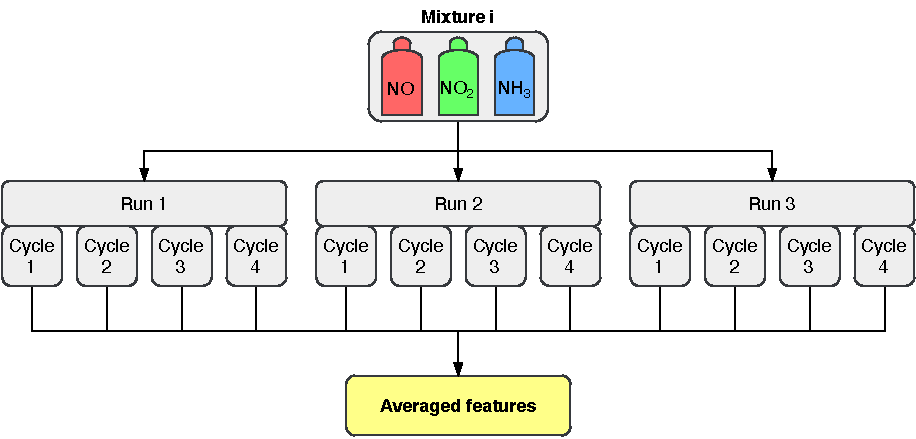
\includegraphics[width=1\textwidth]{../figures/averaging-process.pdf}
	\caption{A visualization of the feature averaging process.}
	\label{fig:averaging-process}
\end{figure}


\begin{table}
	\centering
	\caption{Sample of averaged features throughout all exposures data.}
	\label{tab:prepro-sample-unique-mixtures}
	\resizebox{\textwidth}{!}{%
		\begin{tabular}{ccp{0.8cm}p{0.8cm}p{0.8cm}p{1.6cm}p{1.6cm}p{1.6cm}p{0.3cm}p{1.6cm}p{1.6cm}}
			\toprule[0.5mm]
			Index &  UNIQUE MIXTURE &    NO &   NO2 &   NH3 & 0.05-1-avg-0 &  0.05-1-avg-1 &  0.05-1-avg-2 & $\dots$&  5000.0-1-avg-238 &  5000.0-1-avg-239 \\
			\midrule[0.5mm]
			0 &         0 &  5.0 &  5.0 &   5.0 &  28.983749 &     25.442410 &     25.383750 &$\dots$&           35.162932 &         35.152458 \\
			1 &         1 &  5.0 &  5.0 &  10.0 & 28.538652 &     24.933269 &     24.879247 &$\dots$&           34.622460 &         34.623591 \\
			2 &         2 &  5.0 &  5.0 &  20.0 & 29.038925 &     25.245278 &     25.181935 &$\dots$&           35.025637 &         35.023103 \\
			3 &         3 &  5.0 &  5.0 &  40.0 &  28.698684 &     25.057399 &     24.980686 &$\dots$&           34.575699 &         34.576649 \\
			4 &         4 &  5.0 &  5.0 &  80.0 & 28.738748 &     25.289980 &     25.229714 & $\dots$&          34.860040 &         34.854340 \\
			\bottomrule
			&&&&&&&&&&\\
			&&&&&&&\sbox0{\dots}\makebox[\wd0]{\vdots}&&&\\
			&&&&&&&&&&\\
			\toprule
			
			70 &        70 &  20.0 &  80.0 &   5.0 &  28.142217 &     24.646824 &     24.596195 &$\dots$&         34.208650 &         34.213536 \\
			71 &        71 &  20.0 &  80.0 &  10.0 &  28.615026 &     24.952453 &     24.893228 &$\dots$&         34.511972 &         34.497900 \\
			72 &        72 &  20.0 &  80.0 &  20.0 &  28.432463 &     24.705665 &     24.649538& $\dots$&         34.317554 &         34.313437 \\
			73 &        73 &  20.0 &  80.0 &  40.0 &  28.327675 &     24.725143 &     24.685825 &$\dots$&         34.213989 &         34.197429 \\
			74 &        74 &  20.0 &  80.0 &  80.0 &  28.611836 &     25.056652 &     24.993128 &$\dots$&         34.592507 &         34.593548 \\
			
			\bottomrule
			&&&&&&&&&&\\
			&&&&&&&\sbox0{\dots}\makebox[\wd0]{\vdots}&&&\\
			&&&&&&&&&&\\
			\toprule
			
			120 &       120 &  80.0 &  80.0 &   5.0 &      28.548244 &     25.157684 &     25.103051 &$\dots$&         34.742313 &         34.749349 \\
			121 &       121 &  80.0 &  80.0 &  10.0 &    28.630183 &     25.045884 &     25.015773 & $\dots$&        34.678857 &         34.675690 \\
			122 &       122 &  80.0 &  80.0 &  20.0 &  28.420835 &     24.737087 &     24.687996 & $\dots$&        34.354338 &         34.347416 \\
			123 &       123 &  80.0 &  80.0 &  40.0 &  28.457189 &     24.743263 &     24.682929 &$\dots$&         34.327938 &         34.319839 \\
			124 &       124 &  80.0 &  80.0 &  80.0 &    28.615161 &     25.093255 &     25.046698 & $\dots$&        34.743829 &         34.734124 \\
			\bottomrule[0.5mm]
	\end{tabular}}
\end{table}


\begin{figure}[!htb]
	\centering
	
	\begin{subfigure}[b]{1\textwidth}
		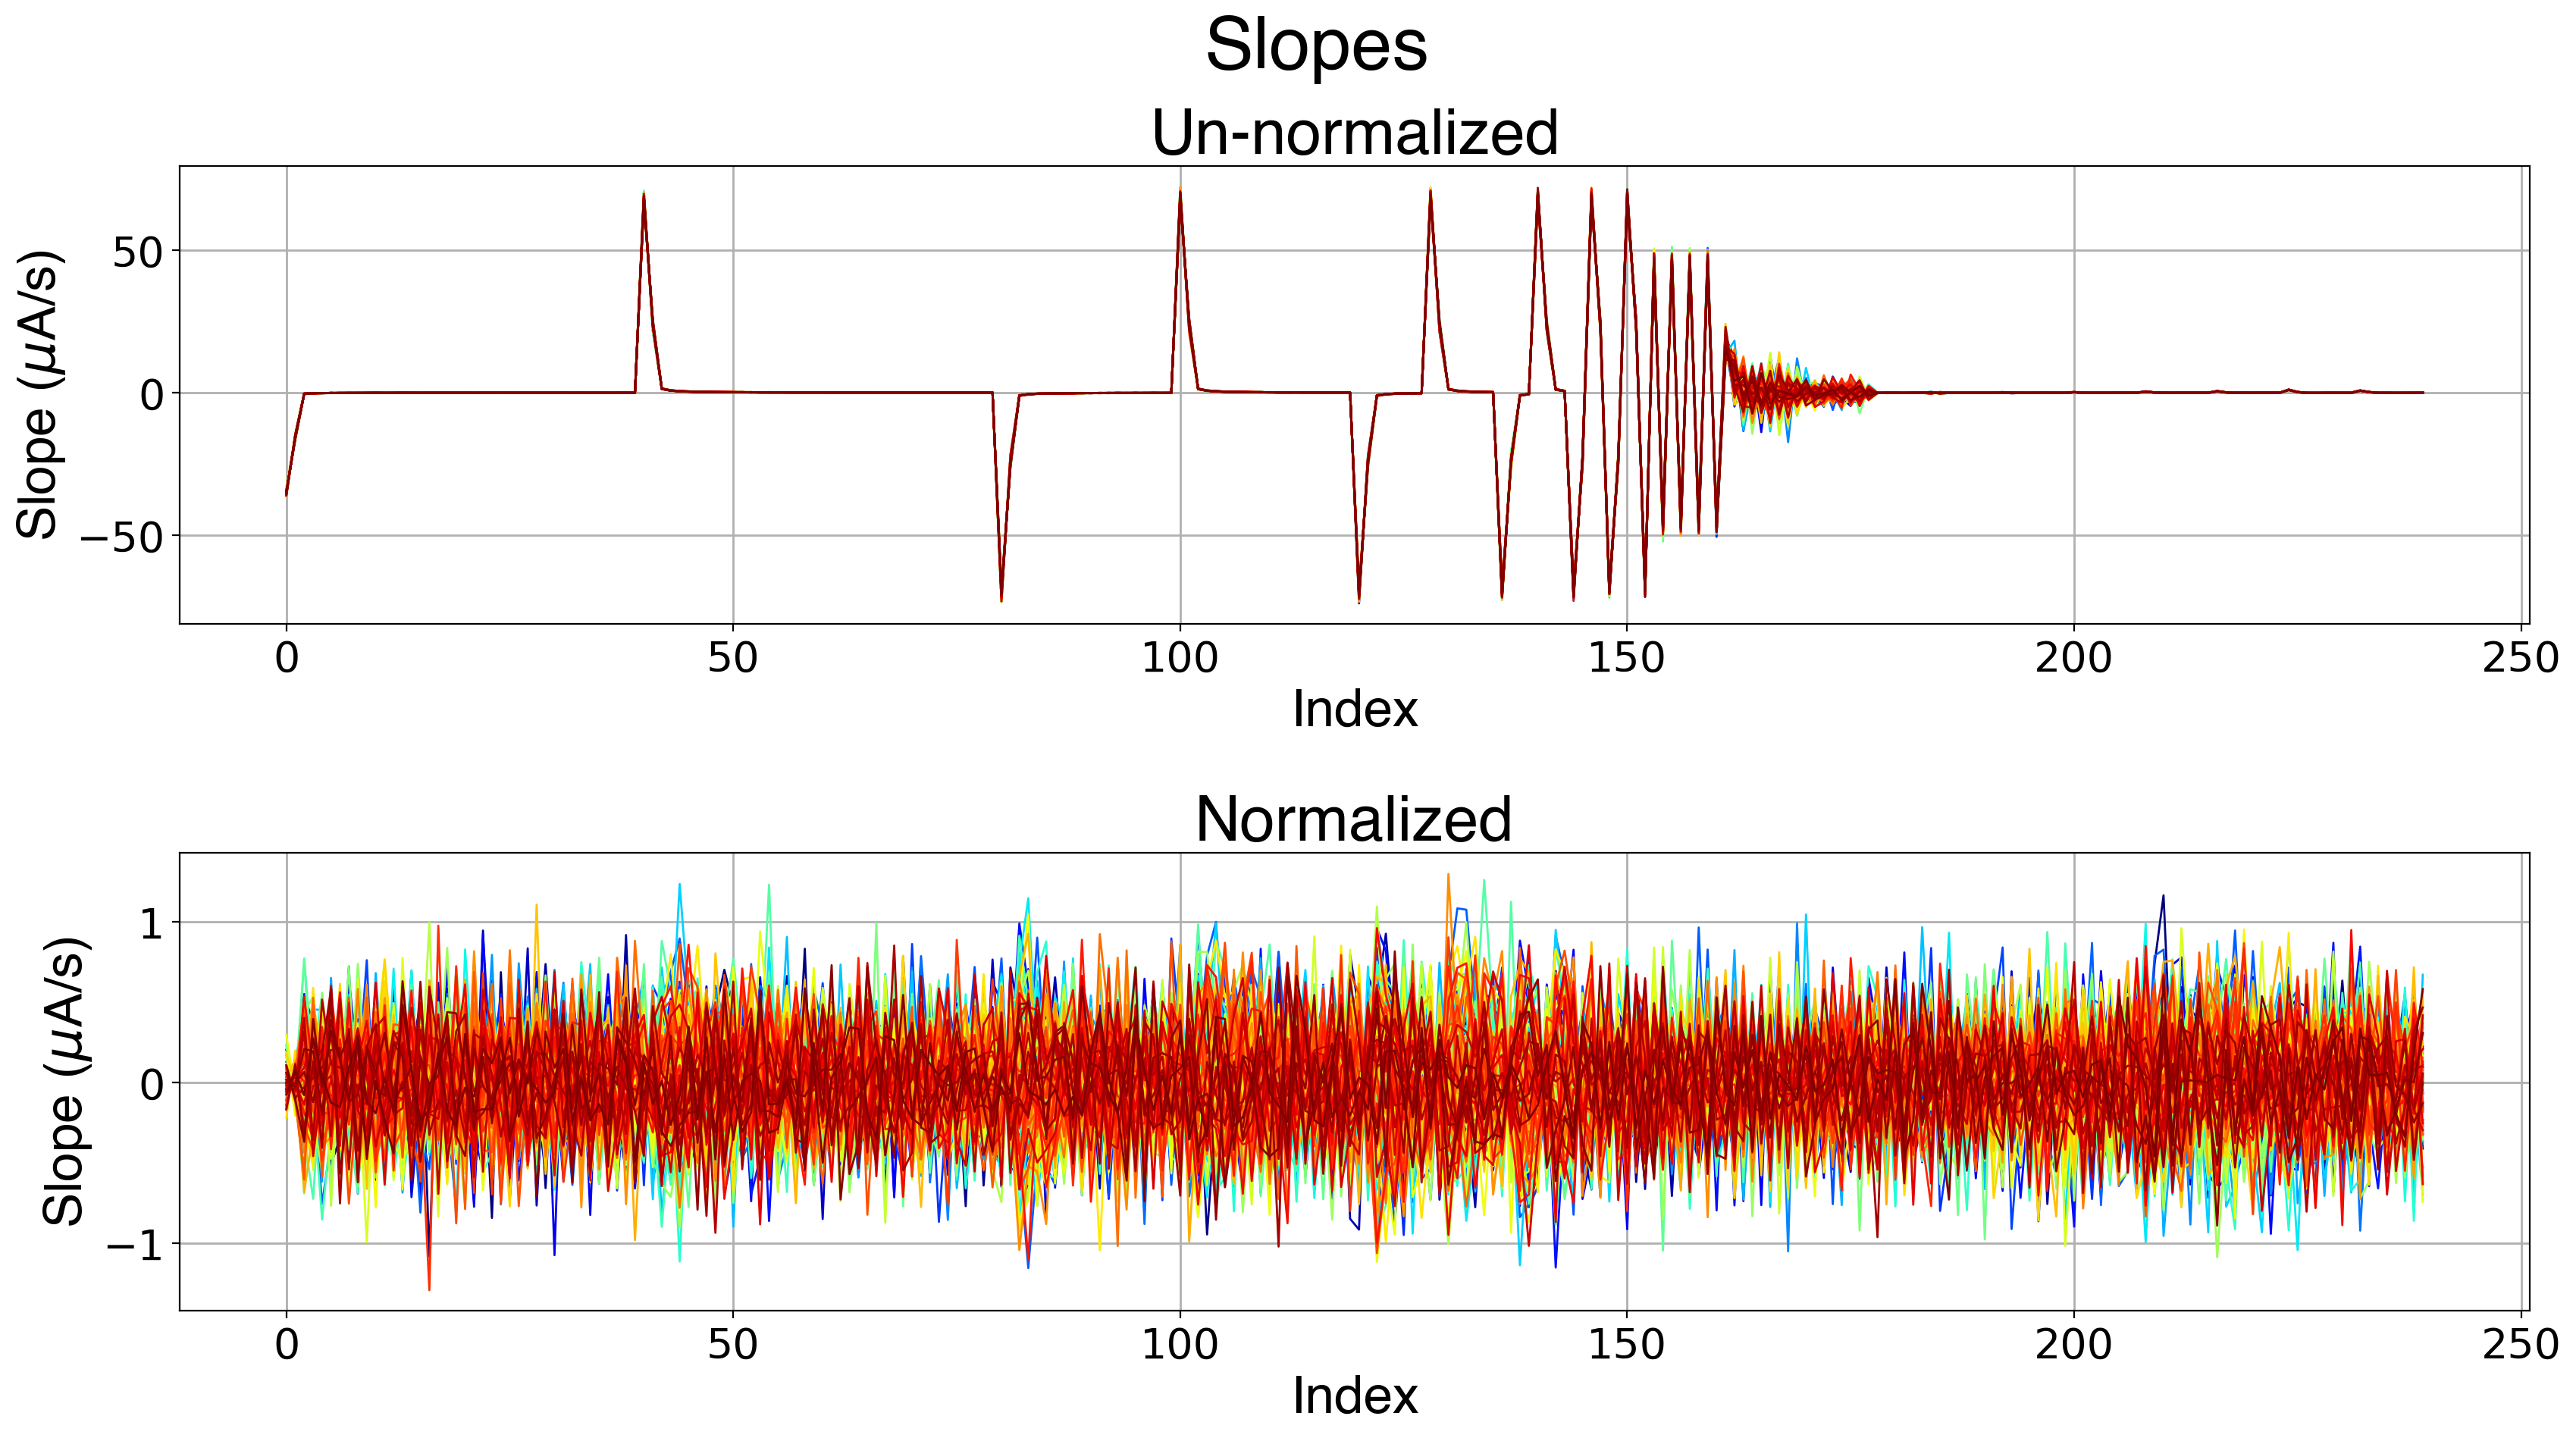
\includegraphics[width=1\linewidth]{../figures/slopes.png}
		\caption{}
		\label{fig:slopes} 
	\end{subfigure}
	
	\begin{subfigure}[b]{1\textwidth}
		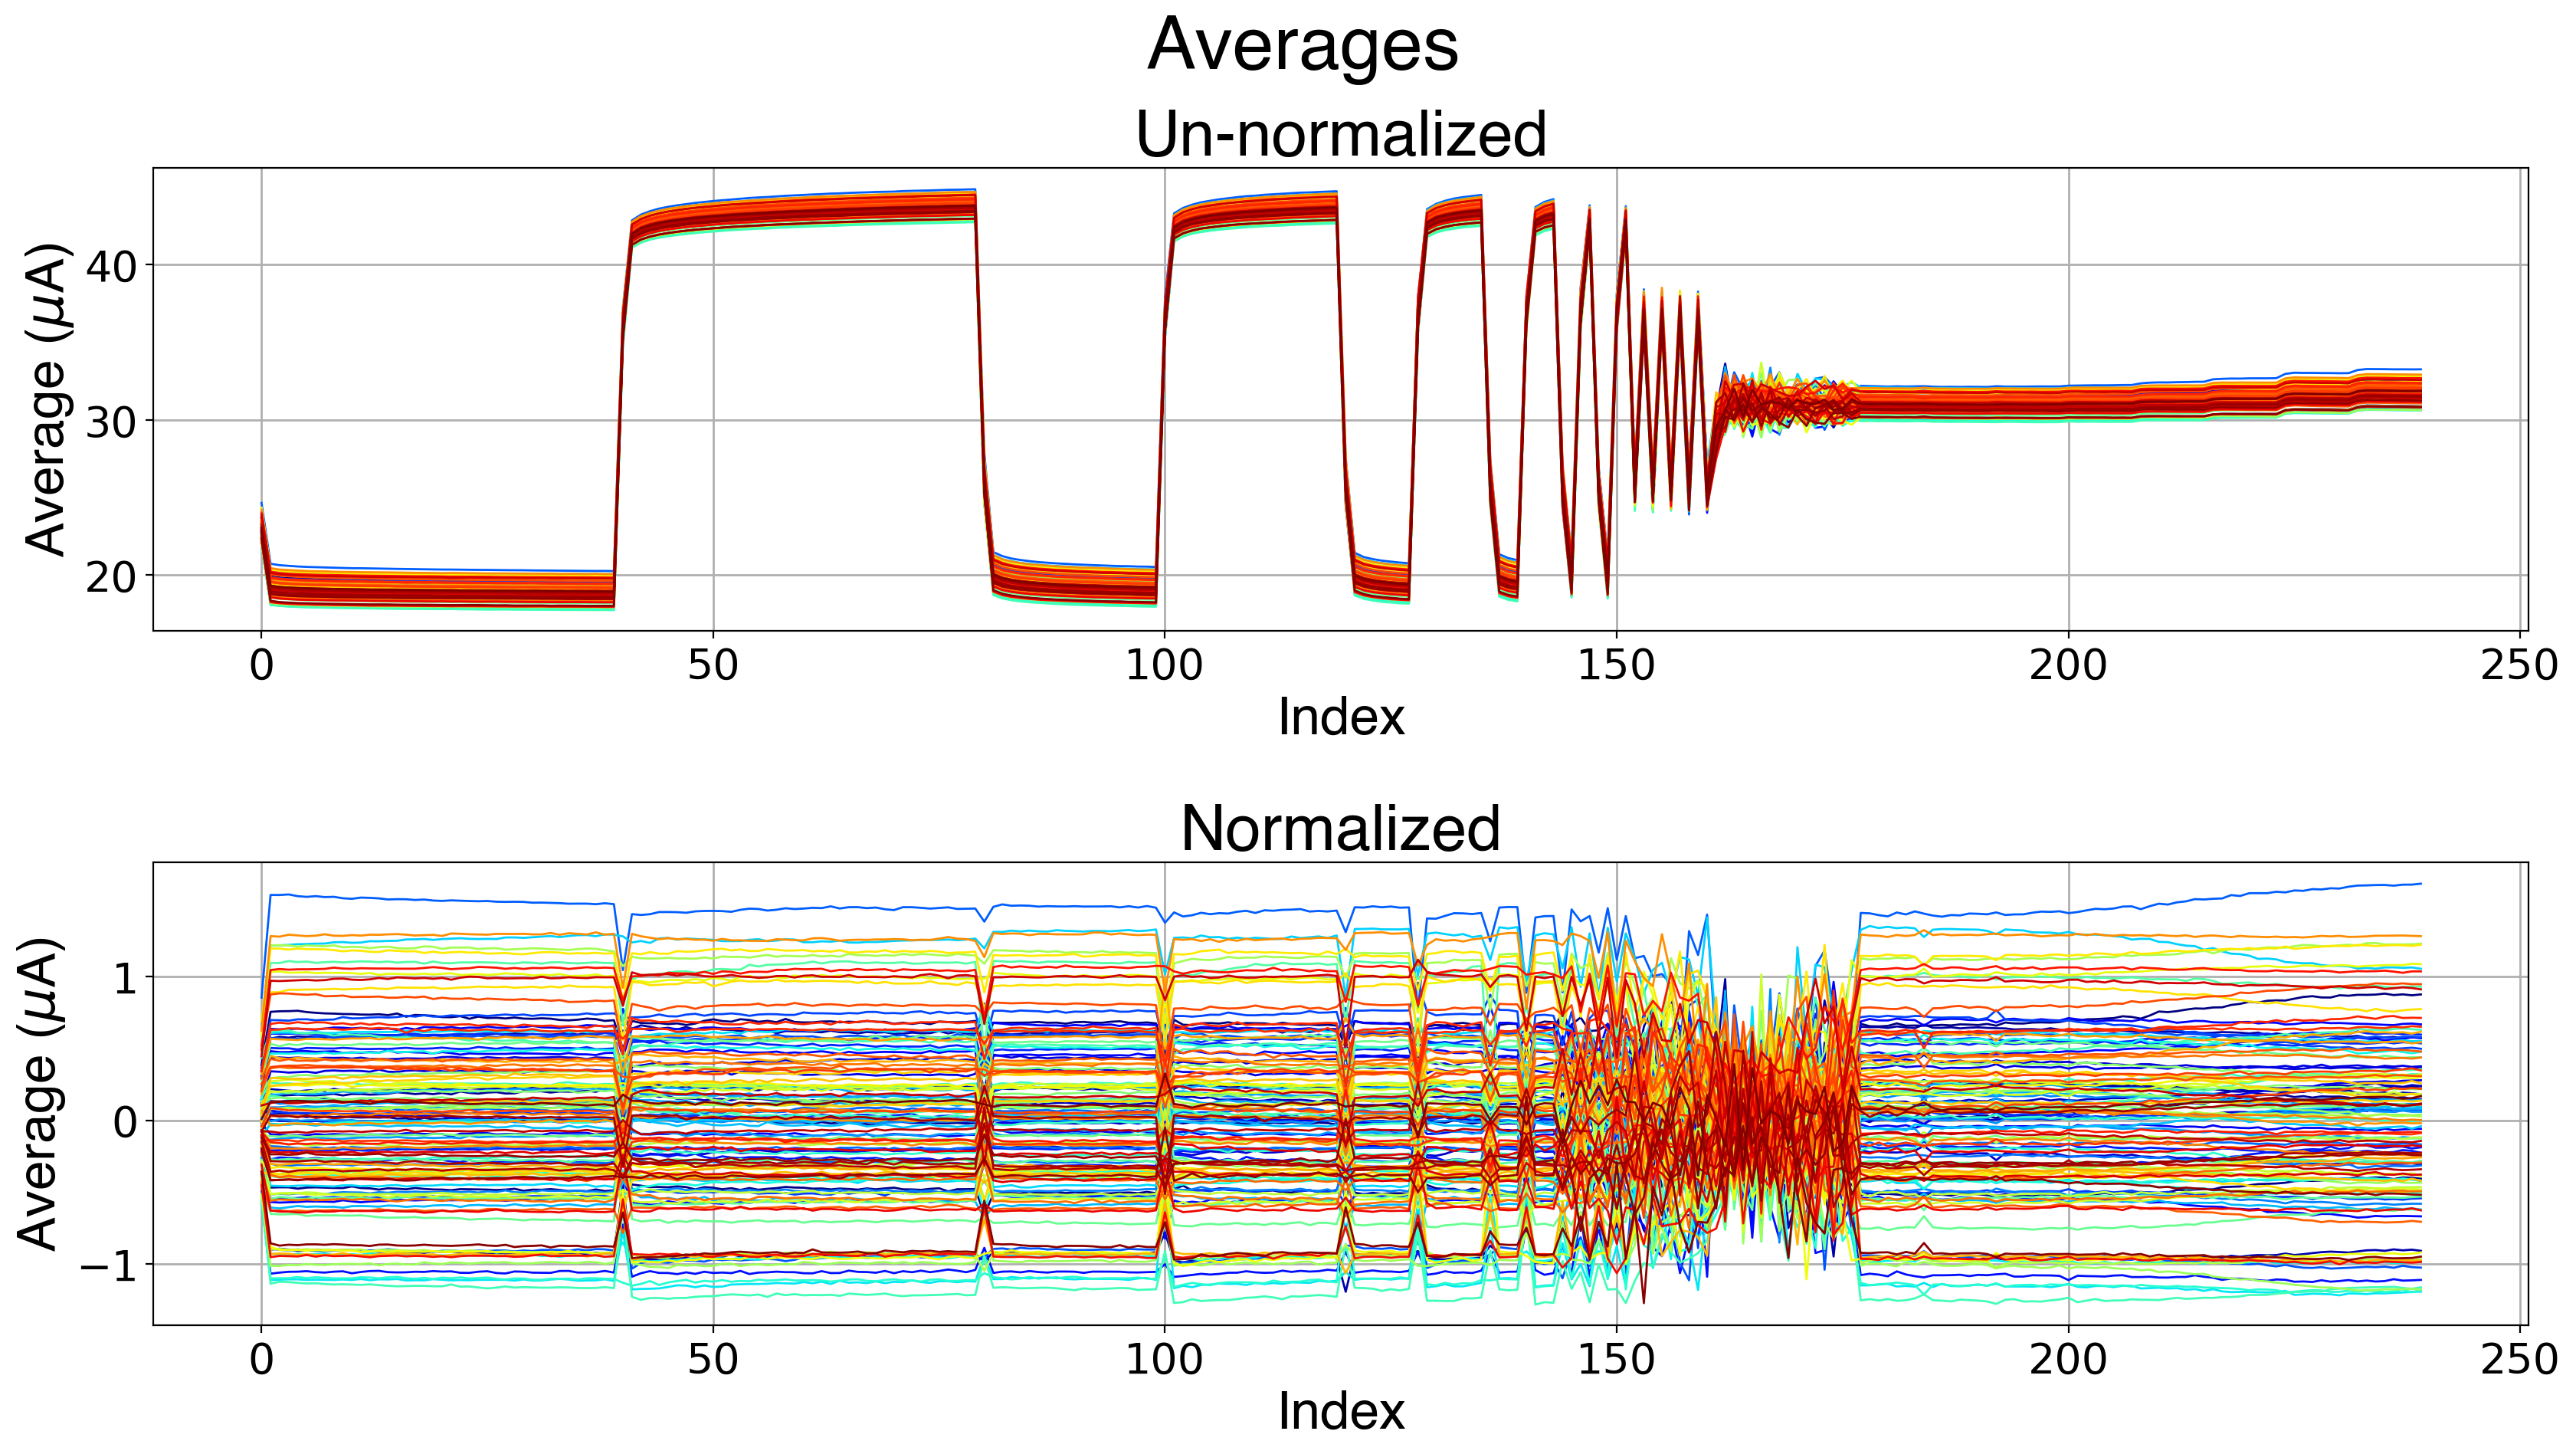
\includegraphics[width=1\linewidth]{../figures/averages.png}
		\caption{}
		\label{fig:averages}
	\end{subfigure}

	\caption{(a) Slope and (b) average features, both un-normalized and normalized.}
	\small
	In each plot, each line represents an unique gas mixture.
	\label{fig:slopes-and-averages}
\end{figure}





